
\subsection{EXT4 文件系统的实现过程}

\subsubsection{LA 体系下 FAT32 与 EXT4 的区别}

首先,我们先介绍一下 EXT4 文件系统:

\begin{center}
    \textit{首先,我们先来介绍一下 EXT4 文件系统的参数:}
    \begin{table}[htbp]
        \begin{tabular}{|c|c|c|c|c|}
            \hline
            文件系统大小 & 单个文件大小 & 子目录可伸展性 & 索引节点 & 碎片整理方式 \\
            \hline
            1 EB & 16 TB \& 48b Bloc_Addr & $\infty$ & 纳秒节点 & 多块分配 + Extends 减少碎片产生 \\
            \hline
        \end{tabular}
    \end{table}
\end{center}

\begin{enumerate}
    \item \textit{与指令集相关:}
    通过分析,我们发现可能有以下几种与指令集相关可能产生影响的因素
    \begin{itemize}
        \item \textbf{LoongArch 架构对于优先级的定义不同:} LoongArch 对于优先级的定义由 PVL0 ~ PVL3 ,其中运行于he'xin'tai
    \end{enumerate}
    \item \textit{与 NPUcore 相关:}
    % INPROCESS
\end{enumerate}

\subsubsection{敲定实现方式}

我们参考了历年不同赛道的优秀作品,最后给出了如下的适配方式:

\textit{我们采用第三方包将稳定 C 库作为外部库调入 NPUcore 中,如下图所示:}

\begin{table}[htbp]
    \centering
    \begin{tabular}{|c|c|}
        \hline
        选用技术栈 & 作用 \\
        \hline
        lwext4 & 稳定的 ext4 文件系统外部库 \\
        bindgen & rust-lang 官方开发的FFI生成工具 \\
        \hline
    \end{tabular}
    \caption{选用技术栈}
\end{table}

\newpage

\begin{figure}[htbp]
    \centering
    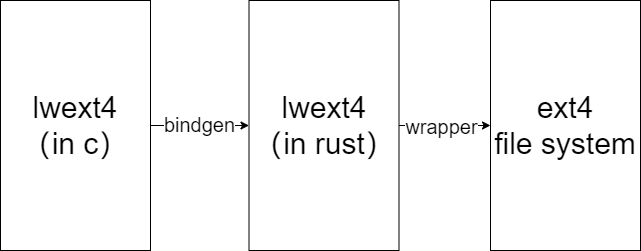
\includegraphics[width=0.6\linewidth]{figs/plan-ext.png}
    \caption{ext4 实现结构图}
    \label{ext4-complexe}
\end{figure}

\begin{enumerate}
    \item \textit{根据 lwext4 或者类似的库理清楚他的函数调用,必要的话给出一个 .h 文件用于包装函数入口:} \\ \textit{The wrapper.h file will include all the various headers containing declarations of structs and functions we would like bindings for. In the particular case of bzip2, this is pretty easy since the entire public API is contained in a single header. For a project like SpiderMonkey, where the public API is split across multiple header files and grouped by functionality, we'd want to include all those headers we want to bind to in this single wrapper.h entry point for bindgen.}\footnote{参考 bindgen 手册https://rust-lang.github.io/rust-bindgen/tutorial-2.html},这意味着,\textbf{对于一个比较复杂而分散的项目,我们最好给出一个包装文件}.
    \item \textit{对于转换完成的rs库,视情况给出rust调用}
    \item \textit{转换我们的fs适配新的rs库} \\ 这部分很简单,我们相当于已经拿来一个ext文件系统了,剩下的就是直接使用调用就行了。在makefile里和rust代码里加入feature就可以做到针对不同文件系统的编译与运行
\end{enumerate}

\vspace{1em}

对于其中可能出现的问题,可见如下列表:

\begin{enumerate}
    \item \textbf{移植的时候会不会出现不适配龙芯情况:}99\%不会,目前查出来 Bindgen 使用 Clang 对 C 文件进行编译,之后反编译(\textit{仅使用 Clang ,不使用 LLVM 编译为机器码})回 Rust ,所以生成的代码最后编译时间还是走的 make 中的 loongarch-gcc .具体编译环节的参考如下:https://blog.csdn.net/xhhjin/article/details/81164076
    \item \textbf{lwext4 的水平如何,是否会存在包本身的问题:} C 语言库,方便阅读;稳定性比较强,多平台测试过,支持小端序,测试过的架构有 x86/AMD64 , ARM 系列以及其的各种嵌入式架构
\end{enumerate}

\subsubsection{第一次适配(LWEXT4-C + Bindgen)}

在第一次适配中,我们试图通过上述方式完成 EXT4 文件系统对于 LA 的适配,然而,我们遇到了许多问题
\begin{enumerate} 
    \item \textit{no_std 环境问题:}我们发现,离开了标准 C 环境的 lwext4 的适配情况并没有我们想象的顺利。在一步步 debug 的过程中,我们经历了如下问题:
    \begin{figure}[htbp] 
        \centering 
        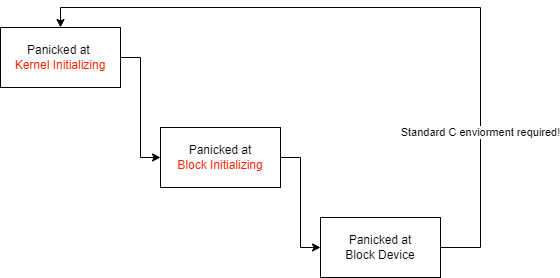
\includegraphics[width=0.5\linewidth]{figs/ext4c.png} 
        \caption{Debug 流程图} 
        \label{debug-ext4c} 
    \end{figure} 
    %\item \textit{工作量问题:}我们试图向内核中添加 C_std 环境,但是由于较大的工作量失败了
\end{enumerate}

\subsubsection{第二次适配(LWEXT4-RUST)}

经过一定时间的查找资料,我们发现了下一个 lwext4 库,其 Supported Features 具体如下:\footnote{github网址:https://github.com/elliott10/lwext4_rust},然而这个包的适配过程仍然十分艰难:

\begin{itemize}
    \item lwext4_rust for x86_64, riscv64 and aarch64 on Rust OS is supported
    \item File system mount and unmount operations
    \item Filetypes: regular, directories, softlinks
    \item Journal recovery \& transactions
    \item memory as Block Cache
\end{itemize}

由于在其 Dependences 中发现了如下信息:

\begin{center}
    \textbf{C musl-based cross compile toolchains}
    \begin{itemize}
        \centering
        \item x86_64-linux-musl-gcc
        \item riscv64-linux-musl-gcc
        \item aarch64-linux-musl-gcc
    \end{itemize}
\end{center}

\textit{我们认为,其在我们拥有 LA 相关工具链的情况下是可以适配至我们的 LA 指令集操作系统上的}

经过一段时间的分析,我们认为 lwext4 系列的库\textbf{由于一定原因与 LA 指令集并不适配}

\subsubsection{第三次适配()}

\subsubsection{第四次适配()}